\documentclass[a4paper,12pt]{article}

\usepackage[utf8]{inputenc}
\usepackage[T1]{fontenc}
\usepackage[spanish]{babel}
\usepackage{caption}
\usepackage{amsfonts, amsmath, amssymb, enumitem, authblk, times, framed, varwidth, graphicx, placeins, indentfirst, pdfpages, fancyhdr, titling, listings} 
\usepackage{float}
\usepackage[justification=centering]{caption}
\setlength{\textwidth}{180mm}
\setlength{\textheight}{250mm}
\setlength{\oddsidemargin}{-10mm}
\setlength{\evensidemargin}{15mm}
\setlength{\topmargin}{-10mm}

\renewcommand{\baselinestretch}{1.4}
\renewcommand{\headrulewidth}{0.5pt}

\lhead{\begin{picture}(0,0) \put(0,0){
\includegraphics[width=20mm]{./LogoITBA}} \end{picture}}
\renewcommand{\headrulewidth}{0.5pt}

\def\FIG#1#2{%
	{\centering#1\par}
	#2}

\pagestyle{fancy}

\begin{document}
	
	\begin{titlepage}
		\centering
			{
\includegraphics[width=0.50\textwidth]{LogoITBA}\par}
			{\bfseries\LARGE Instituto Tecnol\'ogico de Buenos Aires \par}
			\vspace{2cm}
			{\scshape\Huge MapReducing Parking Tickets \par}
			\vspace{0.5cm}
			{\itshape\Large 72.42 Programación Orientada a Objetos - 2024Q1 \par}
			\vspace{1cm}
			
			{\Large \textbf{\underline{Alumnos:}} \par}
			{\Large \large \textbf{Tomás Santiago Marengo}, 61587 \par}
			{\Large \large \textbf{Abril Occhipinti}, 61159 \par}	
			{\Large \large \textbf{Santino Ranucci}, 62092 \par}	
			{\Large \large \textbf{Agustin Zakalik}, 62068 \par}	
			
			\vspace{1cm}
			
			{\Large \textbf{\underline{Profesores:}} \par}
			{\Large \large \textbf{Ing. Marcelo Turrín} \par}
			{\Large \large \textbf{Ing. Franco Román Meola} \par}		
			
			\vfill
	\end{titlepage}
	
	\newpage
	\tableofcontents
	\newpage
	
	\section{Introducción}
	
	En este trabajo, se explora el diseño y la implementación de un sistema distribuido utilizando Hazelcast y el paradigma MapReduce para procesar grandes volúmenes de datos de infracciones de tránsito. El objetivo principal es desarrollar consultas eficientes y escalables, optimizando el rendimiento y evaluando estrategias de procesamiento distribuido. Se tomaron decisiones críticas en la arquitectura del sistema para maximizar la eficiencia y minimizar la latencia, evaluando alternativas de diseño con base en la escalabilidad y robustez.
	
	\bigskip
	
	Se analizó el impacto de utilizar, o no, combiners, de diferentes implementaciones y se realizaron pruebas con conjuntos de datos variados, para probar cómo esto afecta el rendimiento. Estos experimentos permiten obtener una comprensión más profunda de cómo diferentes factores influyen en la eficiencia del procesamiento distribuido.
	

	\newpage
	
	\section{Diseño de los componentes de cada MapReduce}
	
	\subsection{Elección de la Key del Mapa Inicial}
	
	En el diseño de un sistema MapReduce, \textbf{la elección de la clave (key) para el mapeo inicial es fundamental para asegurar una distribución equilibrada de la carga entre los nodos}. La clave debe ser seleccionada teniendo en cuenta la naturaleza del dataset para evitar sobrecargar un solo nodo. En un escenario ideal con un número considerable de nodos, la distribución equitativa de los datos es crucial.
	
	\bigskip 
	
	Como ejemplo, para la consulta de las top 3 infracciones por barrio, inicialmente podríamos pensar en utilizar el barrio como clave. Sin embargo, esta elección puede llevar a una distribución desigual si ciertos barrios concentran un alto porcentaje de las infracciones. Por ejemplo, en un dataset de infracciones de tránsito en una gran estado, algunas ciudades de mayor concentración demográfica o  industrial, pueden tener una mayor densidad de población y, por lo tanto, más infracciones. Si el barrio se utiliza como clave, los nodos que procesan esos barrios podrían sobrecargarse. El tiempo en un proceso en paralelo es el tiempo del que más tarda, por lo que en el peor caso podría ser como no distribuir la data.
	
	\bigskip
	
	Para evitar este problema, \textbf{se decidió utilizar una clave primaria (PK) autoincremental} como clave para la distribución de los datos. Esto asegura que los tickets se distribuyan aleatoriamente entre los nodos, equilibrando la carga de trabajo. Sin embargo, dependiendo de la naturaleza de la agrupación requerida por la consulta, puede requerir una etapa adicional de procesamiento para agrupar los datos de interés.
	
	\subsection{Componentes}
	
	Primero se detalla la idea general, que en principio valdría para cualquier consulta, salvo excepciones. En tal caso se nombrarán aparte.
	
	\bigskip
	
	Los \textbf{mappers} toman cada ticket con un ID particular y emiten pares clave-valor en la forma (clave de interés, 1). Cada ticket se sube a la red con la información pertinente para cada consulta. Esto es simplemente para agilizar los testeos y no sobrecargar la red, aunque se entiende que en un ambiente operativo y del día a día estos datos ya están cargados.
	
	\bigskip
	
	Los \textbf{combiners} realizan una operación similar a la de los reducers pero a nivel local en cada nodo. Agrupan los valores (1s) localmente para reducir la cantidad de datos que necesitan ser transferidos a través de la red en la fase de reducción.
	
	\bigskip
	
	Los \textbf{reducers} agrupan los valores recibidos de los mappers y combiners, sumando los 1s para cada clave de interés. Este proceso consolida los datos a nivel global.
	
	\bigskip
	
	Los \textbf{collators} trabajan con un orden de magnitud mucho menor después de la fase de reducción, realizando operaciones finales como el ordenamiento y selección de los top N elementos que son poco costosas dada la magnitud de la información que le llega, pero no es siempre así...
	
	\subsubsection{¿Y si el collator trabaja con mucha información?}
	
	En el caso de la Query 4, que requiere encontrar las placas de peor comportamiento por barrio, el orden de magnitud de los datos que llegan al collator es considerablemente alto. Los datos están compuestos por pares (barrio, placa), donde la cantidad de barrios es relativamente pequeña pero la cantidad de placas puede ser muy grande.
	
	\bigskip
	En ese caso hay dos opciones: 
	
	\begin{enumerate}
		\item Para manejar este gran volumen de datos, se puede realizar un MapReduce adicional. Si el collator recibiera un dataset con un orden de magnitud muy alto, el procesamiento se volvería ineficiente, por ejemplo un ordenamiento sería muy costoso. Por lo tanto, se optó por dividir el trabajo en dos fases de MapReduce.
		\item Se puede pensar desde cero el MapReduce, utilizando otra key que no sea el entero incremental, y que permita reducir la magnitud de la información en pasos anteriores como el mapper o el reducer.
	\end{enumerate}

	\subsubsection{¿KeyPredicate?}
	
	En este caso no usamos KeyPredicate porque este sirve para filtrar por las keys y las queries no pedían nada de filtrado previo que pueda ser usado en claves. Existe un filtrado de fechas para la Query 4 pero este se realiza en el Mapper para no emitir cosas de más. Se podría haber utilizado si se pidiera un filtrado como por ejemplo ``los barrios pero que empiecen con A'', en ese caso podría haber estado bueno utilizar barrio como key.
	
	\subsection{Queries}
	
	A continuación se resume la lógica de cada query, recordando que resuelve cada una.
	
	\subsubsection{Query 1}
	
	La consulta 1 es bastante simple. Pide el total de multas por infracción (definición). 
	
	\begin{enumerate}
		\item El mapper emite (definición, 1).
		\item El combiner simplemente suma lo que el mapper le mandó por cada definición, emite (definición, suma).
		\item El reducer hace exactamente lo mismo que el combiner pero a nivel global.
		\item El collator entrega el resultado final en un TreeSet para ser iterado y escrito en el CSV de salida.
	\end{enumerate}

	\subsubsection{Query 2}
	
	La consulta 2 pide top 3 infracciones más populares de cada barrio. En la sección 3.3 se menciona una colección propia que implementamos para esta query. Esta query si bien pide el top 3, se le puede pasar el mismo parámetro ``Dn='' y que sea cualquier tipo de top.
	
	\begin{enumerate}
		\item El mapper emite (<barrio, definición>, 1).
		\item El combiner simplemente suma lo que el mapper le mandó por cada par, emite (<barrio, definición>, suma).
		\item El reducer hace exactamente lo mismo que el combiner pero a nivel global.
		\item El collator entrega el resultado final en un TreeSet para ser iterado y escrito en el CSV de salida. Utiliza TopNSet para ordenar las infracciones por barrio.
	\end{enumerate}

	\subsubsection{Query 3}
	
	La consulta 3 pide top N agencias con mayor porcentaje de recaudación.
	
	\begin{enumerate}
		\item El mapper emite (agencia, monto).
		\item El combiner simplemente suma lo que el mapper le mandó por cada agencia, emite (agencia, sumaMonto).
		\item El reducer hace exactamente lo mismo que el combiner pero a nivel global.
		\item Debido que el orden de magnitud de la información que recibe el collator no es tan grande (cantidad de agencias), este se encarga de calcular los porcentajes sobre el total del monto.
	\end{enumerate}

	\subsubsection{Query 4}
	
	La consulta 4 nos retorna la patente con más infracciones de cada barrio en el rango [from, to]. Esta en primera instancia se hizo con dos MapReduce.
	
	\begin{enumerate}
		\item El mapper1 filtra por el rango de fecha y emite (<patente, barrio>, 1).
		\item El combiner1 simplemente suma lo que el mapper le mandó por cada par.
		\item El reducer1 hace exactamente lo mismo que el combiner1 pero a nivel global.
		\item Esto devuelve la cantidad de veces que existen cada par <patente, barrio>. Como el orden de magnitud es patente $\cdot$ barrio (muy alto) se hace un segundo MapReduce.
		\item El mapper2 emite (barrio, <patente, cantidad>).
		\item El combiner2 emite (barrio, patenteConMasInfracciones).
		\item El reducer2 hace exactamente lo mismo que el combiner2 pero a nivel global.
		\item El collator entrega el resultado final en un TreeSet para ser iterado y escrito en el CSV de salida.
	\end{enumerate}

	\subsubsection{Query 5}
	
	La consulta 5 resuelve los pares de infracciones que tienen, en grupos de a cientos, el mismo promedio de monto de multa.
	
	\begin{enumerate}
		\item El mapper emite (definición, monto).
		\item El combiner emite (definición, <suma, cantidad>). Se necesita la cantidad porque el promedio de los promedios no es el promedio usualmente (solo cuando si la cantidad de todos los combiners es igual, lo cual no es necesariamente cierto).
		\item El reducer ya puede calcular el ``grupo de cien'' y emitir (definición, grupo).
		\item El collator entrega un TreeSet iterable, con los pares de infracciones que son del mismo grupo, sin repetir y en orden alfabético.
	\end{enumerate}

	\newpage
	
	\section{Cuestiones particulares sobre la implementación}
	
	\subsection{Parallel Read}
	
	Para abordar eficientemente la lectura de archivos grandes, optamos por un enfoque secuencial con procesamiento concurrente. Esto significa que utilizamos un solo hilo para leer el archivo CSV línea por línea, colocando cada línea en una cola. Luego, múltiples hilos consumen las líneas de esta cola, procesando y filtrando los campos de interés para luego ser almacenados en el IMap de Hazelcast.
	
	\bigskip
	
	Como resultado directo de esta implementación, logramos reducir significativamente el tiempo de procesamiento de archivos grandes, como por ejemplo, el archivo CSV de NYC con 15 millones de líneas que pasó de más de 1 hora a entre 3 y 4 minutos (que consideramos razonable).
	
	\subsection{Multas de cualquier otra ciudad}
	
	Para ser lo más permisivos posible al leer archivos CSV de diferentes formatos, diseñamos un sistema configurable que permite al usuario definir la estructura del CSV a través de un archivo JSON y manejar diferentes formatos de fecha.
	
	\bigskip
	
	El usuario debe subir un archivo JSON que especifica el índice de cada columna de interés entre los campos mencionados en el trabajo práctico. Esto permite una flexibilidad considerable, ya que el sistema puede adaptarse a diferentes estructuras de archivos CSV sin necesidad de modificar el código fuente. El usuario además puede subir archivos que tengan más columnas y el programa se encargará de tomar sólo las de interés.
	
	\bigskip
	
	Luego, la clase DateFormats permite agregar diferentes tipos de formatos de fecha, facilitando la inclusión de CSV con distintos formatos de fecha. Las fechas suelen variar más que otros campos en los datasets, por lo que esta flexibilidad es esencial.
	
	\bigskip
	
	Para los demás campos optamos por elegir tipos que engloben a lo que se encuentra usualmente. Por ejemplo, para el monto usamos Double, ya que si es entero o con decimales no estamos perdiendo información.
	
	\subsection{TopNSet}
	
	TopNSet es una colección que se encarga de mantener siempre N elementos ordenados para cada key. La idea era usarla para la query 2 y 3, pero al final sólo sirvió para la 2. De esta manera dejamos a la segunda consulta como genérica en vez de ``top 3''. Igualmente para respetar la consulta se pasa como parámetro 3 por defecto.
	
	
	\newpage
	\section{Resultados}
	
	\subsection{Tiempo para cada query según cantidad de nodos}
	
	El siguiente gráfico se generó a partir de los resultados analizados sobre el dataset de 15M de líneas de NYC (el que se encuentra en Pampero). 
	
	\begin{figure}[h!]%
		\FIG{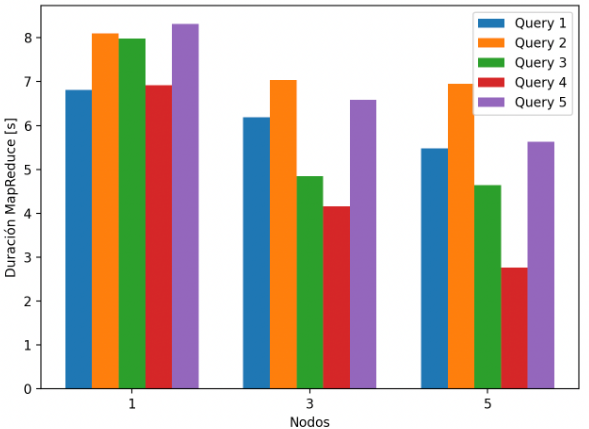
\includegraphics[width=0.75\textwidth]{./queries_vs_nodos.png}}
		{\caption{Tiempo de cada Query con diferente cantidad de nodos}
			\label{fig1}}
	\end{figure}

	Se destaca que:
	
	\begin{enumerate}
		\item La performance aumenta a medida que se agregan más nodos ya que se distribuye el cómputo de la tarea. Sin embargo (hay muchos ``peros'' en este trabajo práctico, pero queremos analizarlos o al menos entenderlos todos), este resultado es así ya que se utilizaron máquinas virtuales en Google Cloud Platform dentro de una misma red privada y muy rápida. 
		
		\item Si esto se hiciera con nuestras computadoras, abriendo puertos y pasando por internet, con ancho de banda muchos menor, al agregar más nodos podría ocurrir que el tiempo de envío de información exceda al tiempo de cómputo, resultando en mayores tiempos para mayor cantidad de nodos. No probamos esta configuración pero hablando con otros grupos notamos eso. En un ambiente productivo se deberían analizar estas cuestiones.
		
	\end{enumerate}
	
	\newpage
	
	\subsection{Con y sin Combiner}
	
	El siguiente gráfico se generó, también, a partir de los resultados analizados sobre el dataset de 15M de líneas de NYC. Pero este se redujo a diferentes tamaños para analizar el cambio de tiempo según se agregaban líneas.
	
	\begin{figure}[h!]%
		\FIG{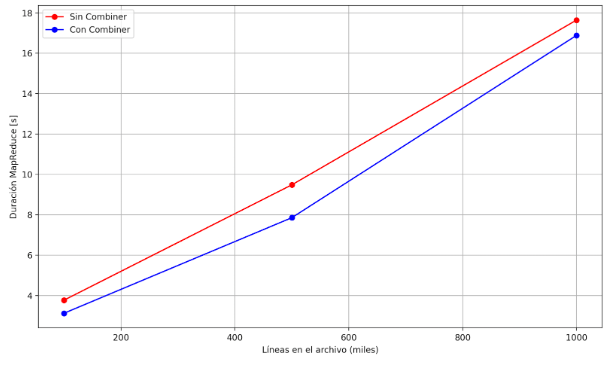
\includegraphics[width=0.75\textwidth]{./con_vs_sin_combiner.png}}
		{\caption{Duración del MapReduce para la Query2 con y sin combiner}
			\label{fig2}}
	\end{figure}

	Con esto podemos notar que claramente hay una diferencia entre tiempos, ya que la idea del Combiner es reducir la información que viaja por la red. Sin embargo, hay que volver a aclarar que esto puede no resultar así. Se destaca lo siguiente:
	
	\begin{enumerate}
		\item En un ambiente local no existe latencia entre el envío de información entre el Combiner y el Reducer, por lo que si estos hacen lo mismo (en diferentes niveles), este cambio en el tiempo de procesamiento no se nota. Casi lo mismo pasa en un ambiente con conexión cableada, que el traspaso de información se hace mucho más rápido que en un ambiente inalámbrico con ancho de banda reducido. Estos resultados nuevamente salen de la misma configuración en GCP.
		
		\item La gráfica muestra (casi) una recta, por lo que a mismo aumento de tamaño del archivo, relativamente mismo aumento de tiempo de procesamiento.
	\end{enumerate}
	
	\subsection{Otra alternativa a la query 4}
	
	Como se mencionó, se usó una PK incremental como key en todas las queries, esto conllevó a que en la query 4 se requieran dos MapReduce debido al orden de magnitud de información que salía del primer Reducer.
	
	Esto desembocó en probar otra configuración, donde el Mapper emite directamente (barrio, patente) en vez de emitir un (<barrio,patente>, 1) y reprocesar algunas cuestiones. 
	
	\begin{figure}[h!]%
		\FIG{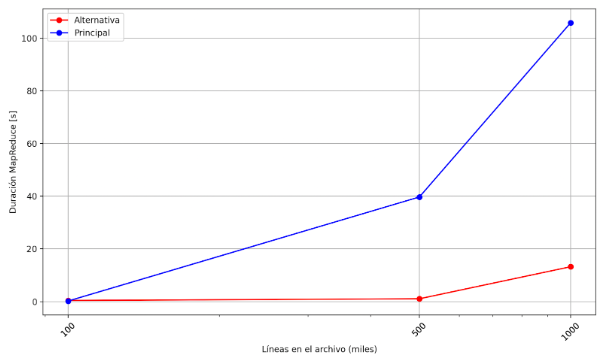
\includegraphics[width=0.8\textwidth]{./query4_alternative.png}}
		{\caption{Comparación alternativa a Query4}
			\label{fig3}}
	\end{figure}

	Se puede ver que hay una mejora sustancial para el método alternativo. Cabe aclarar que estas corridas no se hicieron con la misma configuración de GCP sino que en una única computadora con menor procesamiento y RAM. Se siguió utilizando el dataset de NYC pero con menores cantidades de líneas.

	\bigskip
	
	La alternativa está en la branch main pero se tiene que cambiar a mano en el switch del cliente (ver sección ``Mejoras a futuro'').
	
	\newpage
	
	\section{Mejoras a futuro}
	
	Se nombran algunos puntos de mejora y/o expansión, que se tuvieron en cuenta, pero debido al calendario apretado de junio y que no eran completamente necesarias para las condiciones se dejan como menciones.
	
	\begin{enumerate}
		\item Recibir por parámetro la estrategia a utilizar y crear diferentes estrategias para todas las queries, probando distintas key iniciales para los IMap.
		\item Generar testeos automáticos y eficientes. Que no se vuelvan a cargar los IMap si no es necesario (imitando un ambiente productivo), ya que en nuestro código luego de cada query se hace un clear de los mapas utilizados.
		\item Testear qué tanto cambia en un ambiente inalámbrico haber guardado las infracciones (código, definición) en un IMap. Ya que en realidad no tiene mucho sentido distribuir esa información porque no es tan pesada.
		\item Analizar completamente la naturaleza del dataset. En realidad no es la idea, porque podrían ser infracciones como podrían ser palabras de un diccionario. Esto se nombró varias veces, por ejemplo, sabiendo los porcentajes de infracciones de cada barrio podríamos determinar si es buena idea utilizar ``barrio'' como key en algunas queries, o esto presentaría un desbalanceo.
	\end{enumerate}
\end{document}
